\chapter{Flexibly-conditional generative modelling}
\label{ch:flexible-diffusion}

So far we have introduced diffusion models in both their unconditional and conditional forms. We now turn our attention specifically to flexibly-conditional forms of generative model. 
%
% We have discussed the applications of conditional diffusion models to tasks including text-to-image and text-based image editing. A similarity between these tasks is that we always know in advance what type of data we will condition on at test-time: e.g. for text-to-image we always condition on a text string; for text-based image editing we always condition on a text string and an input image. In other words, the models were trained to work with a single type of conditioning information $\rvy$.
%
Flexibly-conditional models are designed to be robust to settings where we do not know beforehand what form $\rvy$ will take at test-time. This is useful for many applications. Image inpainting settings require the capability to condition on any pixels in an image depending on a user's requirements at test time. For video editing (or video generation from keyframes), a user might need to condition on every second frame, every tenth frame, only the first few frames, or so on. In this chapter we first formalise the idea of a flexibly-conditional generative model~\citep{ivanov2018variational} and review relevant techniques from the literature. We then lay out a concrete strategy for implementing and training flexibly-conditional diffusion models.


\section{Definition}
Ideally we would like to have generative models that need to be trained once and then can be used for \textit{any} conceivable conditioning task at test-time without requiring additional training or data. That is, we would like them to accurately approximate $\pdata(\rvx|\rvy)$ for any possible form of $\rvy$ they are given at test-time and no matter how it is related to $\rvx$. Clearly, though, having a model that can perform \textit{any} conceivable conditioning task is not possible: it wouldn't make sense to train a model on a dataset of images and then expect it to perform text-conditional image generation without ever having seen text data. 
%
% One solution to this is through integration with foundation models~\citep{brown2020language,bommasani2021opportunities}, such as vision-language models~\citep{openai2023gpt,team2023gemini}, which can incorporate common-sense knowledge. We focus instead on methods that do not require additional data sources or foundation models.
%
A more tractable approach, seen in the literature in various forms~\citep{ivanov2018variational,tashiro2021csdi,garnelo2018neural}, is therefore to constrain the set of conditioning tasks as follows. We will consider a flexibly-conditional generative model to be one that, after being trained with data $\rvx \sim \pdata(\cdot)$, can sample $\rvx$ conditioned on the values of any subset of the components of $\rvx$. For an image generative model, if we treat each pixel as a component, this means being able to condition on any subset of the pixel values. For video tasks, we will consider each frame to be a component and so our flexibly-conditional video models can be conditioned on any subset of the frame values.

To restate this with notation from \cref{sec:other-methods-for-conditional-sampling}, we will describe what $n_\rvy$ components to condition on with a set of integer indices $\gY = \{ y_1, \ldots, y_{n_\rvy} \}$. We will then define $\rvy = \rvx[\gY] = [ \rvx[y_1], \ldots, \rvx[y_{n_\rvy}] ]$ as a data structure in which the $i$th element is equal to $\rvx[y_i]$. Different $\gY$ correspond to different conditional generation tasks; each conditional generation task is to generate samples from an approximation of the posterior under the data distribution of $\rvx$ given $\rvy$ and $\gY$
\begin{equation} \label{eq:flexible-diffusion-target}
    \pdata(\rvx | \rvy, \gY) = \frac{\pdata(\rvx)\pdata(\rvy|\rvx,\gY)}{\int \pdata(\rvx)\pdata(\rvy|\rvx,\gY) \mathrm{d}\rvx} 
%    \frac{\pdata(\rvx)\delta_{\rvx[\gY]}(\rvy)}{\int \pdata(\rvx)\delta_{\rvx[\gY]}(\rvy) \mathrm{d}\rvx}
\end{equation}
where $\pdata(\rvy|\rvx,\gY) = \delta_{\rvx[\gY]}(\rvy)$ is a Dirac distribution that enforces $\rvy = \rvx[\gY]$.
In other words, each conditional generation task is to sample data conditioned on observed components and with knowledge of the index of each observed component. 
%
While we focus on modelling modalities separately, the framework described here does, in principle, allow flexibly-conditional generative models to span multiple modalities. If, for example, $\rvx \sim \pdata(\cdot)$ is defined to be an object containing both an image and a text caption, a flexibly-conditional generative model trained on such data would be capable of any of image captioning, text-to-image generation, or unconditional image and caption generation.


\begin{table}[t]
    \centering
    \caption{Comparison of two families of flexible conditioning techniques.}
    \begin{tabular}{l|c|c|c}
        \toprule
        & \shortstack[c]{Exact if neural net. \\ loss is optimal}              & \shortstack[c]{Compatible with \\ fast sampling}      & \shortstack[c]{Avoid specifying \\ task distribution}  \\
        \midrule
        \shortstack[l]{Test-time \\ guidance}                               & \raisebox{0.5ex}{\xmark}     & \raisebox{0.5ex}{\xmark}     & \raisebox{0.5ex}{\checkmark} \\
        \midrule
        \shortstack[l]{Training with \\ broad task \\ distribution}         & \raisebox{2ex}{\checkmark} & \raisebox{2ex}{\checkmark} & \raisebox{2ex}{\xmark}     \\
        \bottomrule
    \end{tabular}
    \label{tab:comparison-flexible-conditioning}
\end{table}

\section{Types of flexibly-conditional generative model}
\paragraph{Flexible conditioning by test-time guidance}
Some types of generative model are naturally amenable to being conditioned in certain ways at test-time, even when trained unconditionally. For example, unconditional autoregressive models are simple to condition on the start of a sequence. For an autoregressive image model, this would usually mean that it is simple to condition on the top of an image but not on the bottom of an image~\citep{van2016pixel}. In the diffusion model setting, some of the conditioning techniques discussed in \cref{sec:other-methods-for-conditional-sampling}, such as the replacement method or reconstruction guidance, are readily applicable at test-time with an unconditional diffusion model. These enabled conditioning on any subset of data components or any linear projection of the data.

As laid out in \cref{tab:comparison-flexible-conditioning}, this approach is convenient but has several disadvantages. The first is that test-time guidance techniques like the replacement method or reconstruction guidance use heuristic approximations in place of the conditional score function $\nabla_{\rvx_t} \log q(\rvx_t|\rvy)$. These can work well in practice but still add another source of error on top of, e.g., imperfections in the learned approximation $\preds(\rvx_t, t) \approx \nabla_{\rvx_t} \log q(\rvx_t)$. Therefore, even if the amount of compute and data used in training the unconditional diffusion model are scaled towards infinity and its loss tends towards the optimum, the guided conditional version will have error that does not tend to zero. The second downside is that, while the replacement method is no slower than unconditional sampling, more advanced techniques like reconstruction guidance are slower since they require gradients to be computed with backpropagation during sampling. In addition, test-time guidance is incompatible with many techniques for reducing the number of step needed in diffusion model sampling such as progressive distillation~\citep{salimans2022progressive}, consistency models~\citep{song2023consistency}, and rectified flow~\citep{esser2024scaling}. Nonetheless using test-time guidance simplifies training by avoiding the need to specify a task distribution, and we will build on these techniques in \cref{ch:tddm}.

\paragraph{Flexible conditioning by training with a broad task distribution}
Generative models including GANs, VAEs, and diffusion models have corresponding conditional variants~\citep{mirza2014conditional,sohn2015learning,tashiro2021csdi} and these can be re-purposed into flexibly-conditional generative models if the information which is conditioned on is varied between training examples~\citep{zhao2021large,ivanov2018variational,tashiro2021csdi}. Doing so requires specifying a broad distribution over tasks for training that covers any desired test-time tasks. We will discuss task distributions further in \cref{sec:flexible-diffusion-objective}, and argue that even very simple choices can enable good performance. 

In return for this effort, explicitly training a flexibly-conditional model yields several improvements over using test-time guidance. One is that it enables conditional generation performance to improve with compute and data without being constrained by approximations like those in test-time guidance. Flexibly-conditional training is also compatible with any techniques for fast-sampling that have conditional variants~\citep{salimans2022progressive,song2023consistency,esser2024scaling}. 

We will give a concrete example of an objective for directly training flexibly-conditional models with the flexibly-conditional diffusion objective presented later in this chapter. We then use it in \cref{ch:fdm} and demonstrate another, related, training objective for flexibly-conditional VAEs in \cref{ch:cigcvae}.

\paragraph{Flexible conditioning by prompting task-agnostic models}
\citet{brown2020language} gave a demonstration of the following recipe. First, they trained a single large language model on task-agnostic data scraped from the internet. Then, at test-time, they would give a specification of a task in natural language. Without any task-specific weight updates or finetuning, the large language model was able to attain good performance on a variety of natural language tasks. More recently, similar models have been trained on multi-modal data that combines natural language with images and sometimes video~\citep{openai2023gpt,team2023gemini,kondratyuk2023videopoet}. This opens the door to future flexible conditioning that is as simple as prompting the model, e.g.: 
\begin{quote}
    ``Generate a video in which the first frame is 〈IMAGE TOKENS〉, the second frame is 〈IMAGE TOKENS〉, and the tenth frame is 〈IMAGE TOKENS〉.''\footnote{In this example, 〈IMAGE TOKENS〉 should be understood as a tokenized representation of the frames we are conditioning on.}
\end{quote}
We are not, though, aware of work which has achieved good results from such a simple technique. A related approach is to use a purely text-based large language model which takes any conditioning information as an input text prompt and outputs a text description of an image or video including, for example, bounding boxes of prominent objects in it. A separate diffusion model can then be conditioned on this text description to generate the image or video~\citep{lian2023llm}. This has been shown to be helpful for tasks in which the conditioning information can be expressed in natural language, but we are not aware of demonstrations of it for tasks like image inpainting or video generation conditioned on certain frames.

\section{Flexibly-conditional diffusion objective} \label{sec:flexible-diffusion-objective}
We now present a training objective and framework for training diffusion models as flexibly-conditional generative models. We do not claim this framework as a novel contribution, in light of its relative simplicity and related work including \citet{tashiro2021csdi,weilbach2023graphically}. Recall that our aim is to approximate the target distribution in \cref{eq:flexible-diffusion-target}. We will denote the approximation of this target from a flexibly-conditional diffusion model as $p_\theta(\rvx|\rvy,\gY)$. To train this flexibly-conditional diffusion model we use the objective
\begin{align} \label{eq:flexible-diffusion-loss}
    \mathcal{L}_\text{FCDM}(\theta) &= \EX_{u(\sigma)u(\gY)q(\rvx, \rvx_\sigma)\delta(\rvy|\rvx,\gY)} \left[ 
    \frac{\lambda^\rvx(\sigma)}{u(\sigma)} \left\| \predx_\theta(\rvx_\sigma, \rvy, \sigma, \gY) - \rvx \right\|_2^2 \right] \mathrm{d}\sigma.
\end{align}
This flexibly-conditional diffusion objective is very similar to the conditional diffusion objective in \cref{eq:cond-diffusion-loss}, with the differences being as follows. First, we now have an expectation over $\gY \sim u(\cdot)$. We will call $u(\gY)$ our \textit{training task} distribution and it is up to the developer of a flexibly-conditional diffusion model to construct it. Second, we now sample $\rvy$ from $\delta(\rvy|\rvx,\gY)$, a Dirac distribution on $\rvy = \rvx[\gY] = [ \rvx[y_1], \ldots, \rvx[y_{n_\rvy}] ]$. One consequence of this manner of sampling $\rvy$ is that it may now have dimensionality that varies between training examples; in fact its dimensionality $n_\rvy$ can now in principle be anywhere between zero and the dimensionality of $\rvx$. Third, we now pass $\gY$ as an extra input into the neural network parameterising $\predx_\theta(\rvx_\sigma, \rvy, \sigma, \gY)$. We will describe how exactly $\gY$ is fed into the neural network for each task in this dissertation as we get to it.

Finally, note that we write the flexibly-conditional diffusion objective in  \cref{eq:flexible-diffusion-loss} as if we are expecting $\predx_\theta(\rvx_\sigma, \rvy, \sigma, \gY)$ to contain predictions for all components of $\rvx$, even components that are specified in $\gY$ and so observed in $\rvy$. In practice a neural network is not needed to make predictions for these components; we can manually implement functionality that copies these values from the input $\rvy$ into the output $\predx_\theta(\rvx_\sigma, \rvy, \sigma, \gY)$. The squared-error loss for such components will then always be zero. The fact that we include them in the squared-error in \cref{eq:flexible-diffusion-loss} is therefore not important in practice.

\paragraph{Sudoku example}
\begin{figure}[t]
    \centering
    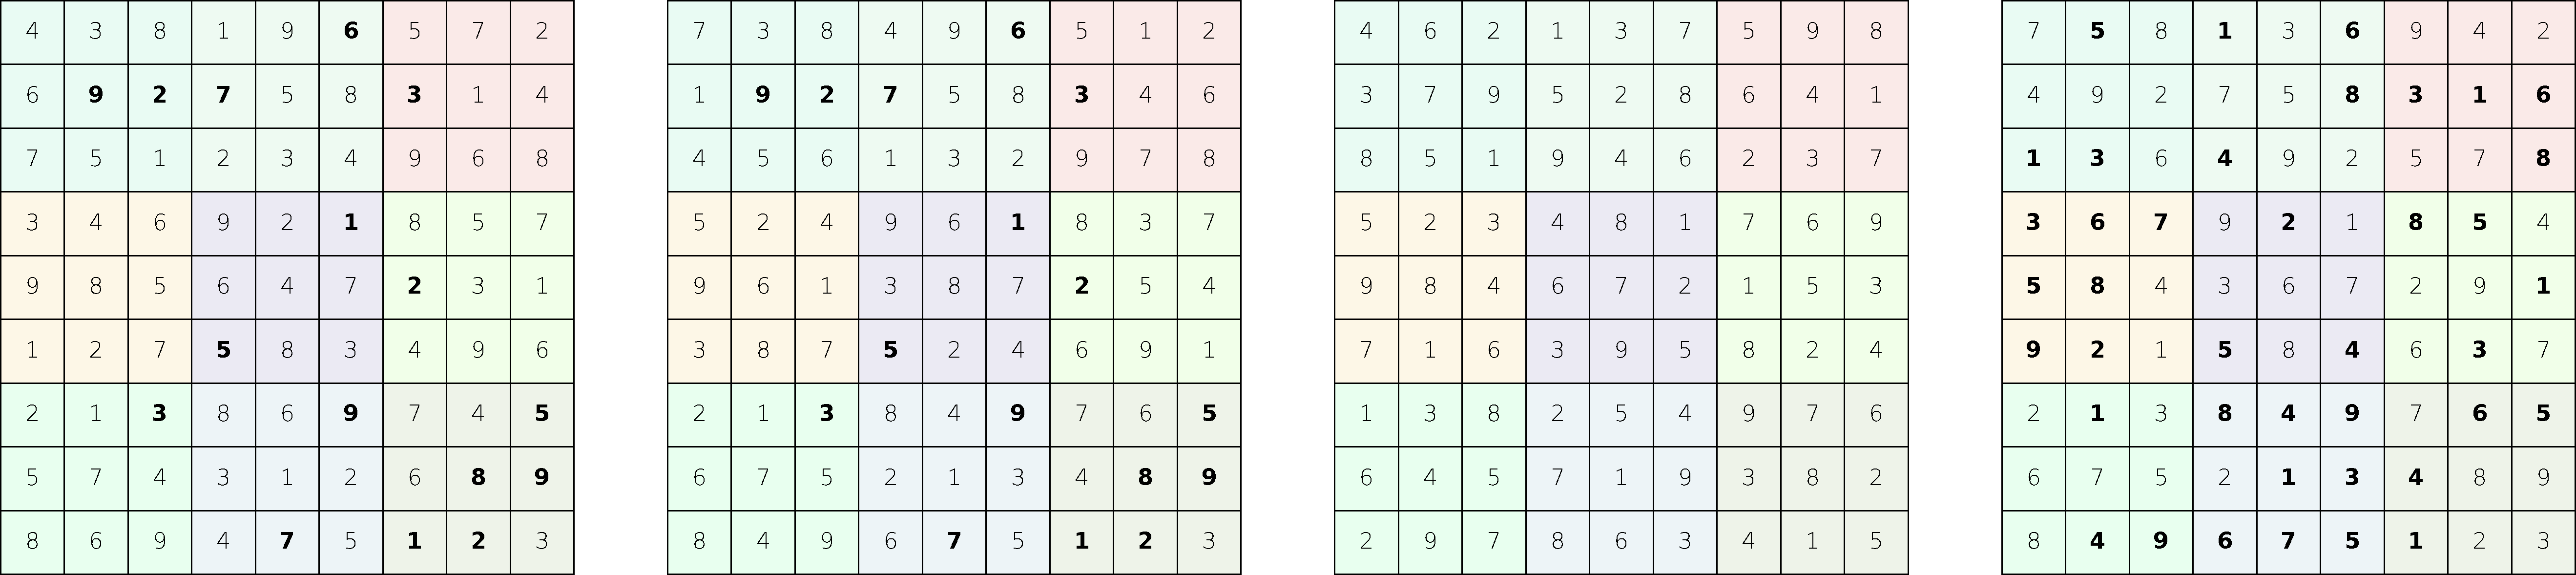
\includegraphics[width=\textwidth]{figs/thesis/sudoku_panel.pdf}
    \caption{Sudoku puzzles solved by a flexibly-conditional diffusion model. Observed numbers (i.e. those that form part of $\rvy$) are shown in bold. The observed numbers are the same for the leftmost two Sudokus but multiple solutions exist, and we show that the model is able to find two different solutions. In the third Sudoku from the left, no numbers were observed. This corresponds to the task with $\gY = \{\}$. The training task distribution $u(\gY)$ covered such tasks and so this flexibly-conditional model is capable of unconditional generation as shown. }
    \label{fig:sudoku-panel}
\end{figure}
We end this section with an intuitive example of a task where flexible conditioning is required: solving Sudoku puzzles~\citep{weilbach2023graphically}. A Sudoku is a $n^2 \times n^2$ grid of integers, each of which takes a value in $\{1,\ldots,n^2\}$. Most commonly, $n$ is set to three so the grid has size $9 \times 9$. There are three types of constraint required for a Sudoku to be valid: no value can appear more than once within the same row of the grid; no value can appear more than once within the same column; and no value can appear more than once within any of the $n^2$ $n \times n$ sub-grids that make up the grid. Sudoku puzzles are puzzles in which the player is required to complete a Sudoku which has missing values. Most puzzles are constructed to have a single solution, but if enough values are missing then multiple solutions can be possible. We can frame solving Sudokus as a conditional generative modelling problem if we have a data distribution $\pdata(\rvx)$ that places probability mass over all complete and valid Sudoku grids.\footnote{Fortunately this distribution is efficient to sample from. We follow the procedure from \url{https://turtletoy.net/turtle/5098380d82}.} The set of observed indices $\gY$ denotes which cells the user is given values for, and the user must infer the values for all cells not in $\gY$. The cells whose values are given as clues vary between different Sudoku puzzles, and so training a conditional generative model that can solve any given Sudoku puzzle means training a flexibly-conditional generative model. 

We trained a flexibly-conditional diffusion model with a very simple training task distribution that uniformly samples how many cells to observe the values of from between zero and $n^4-1$ (the number of cells minus one) and then uniformly samples this many cell indices to construct $\gY$. We process the input to the neural network by replacing elements of $\rvx_\sigma$ corresponding to observed values with those observed values. The network then performs a linear projection of each resulting value and adds a learned embedding to elements with observed values. This forms the input to a transformer-based architecture~\citep{vaswani2017attention}. We refer to \citet{weilbach2023graphically} for further details of the architecture and training procedure. \Cref{fig:sudoku-panel} shows a variety of Sudoku puzzles solved by our flexibly-conditional diffusion model.

\section{Outline of the remaining chapters}
In the chapters that follow we will build on the flexibly-conditional generative modelling framework in several ways. First, in \cref{ch:fdm}, we will define an even more flexible model that is capable of ``marginalising out'' components in the original data that we do not wish to sample or condition on. To do so we will modify \cref{eq:flexible-diffusion-target} to additionally condition on $\gX$, the indices of components we wish to generate and then sample the values of only those $|\gX|$ elements. This will let us scale flexibly-conditional generative models to large and complex data in the form of long videos. In \cref{ch:tddm} we will explore how to build flexibly-conditional generative models for the case where the data has varying dimensionality and $\pdata(\rvx | \rvy, \gY)$ is a trans-dimensional distribution from which different samples can have different dimensionality. In this case, conditioning on $\rvy$ may have an impact on the dimensionality of the data points that the model should sample. In \cref{ch:cigcvae} we will explore how to cheaply train a flexibly-conditional generative model for the image domain based on the variational auto-encoder framework. We end by discussing our final conclusions and outlook in \cref{ch:conclusion}.
